
%\usetikzlibrary{positioning}
%\tikzset{>=stealth}
%
%\newcommand{\tikzmark}[3][]{\tikz[remember picture,baseline] \node [anchor=base,#1](#2) {$#3$};}

\section{Many-particle states, fermions}

\subsection{N-particle vacuum state}



Many-particle states will be built up by constructing a basis using products of single-particle states. 
Let $\lambda$ be some set of quantum numbers that uniquely specifies a single-particle quantum state.\\

\noindent Example: $\lambda$ could be the set of quantum numbers of the hydrogen-atom.\\
$\lambda = (n,l,m, \sigma)$\\
\begin{align*}
	n &: \text{Main quantum number.}\\
	l &: \text{Orbital angular momentum quantum number.}\\
	m &: \text{Quantization of angular momentum along z-axis.}\\ 
	\sigma &: \text{Spin quantum number.}
\end{align*}

\noindent Motion in 3 dimensions $\implies$ 3 quantum numbers : $(n,l,m)$\\
Spin: 1 quantum number.\\

\[ \begin{array}{ll}
\mbox{Corresponding state:} & \ket{n_\lambda}\\
\mbox{Adjoint state:} &  \bra{n_\lambda} = \left(\ket{n_\lambda} \right)^\dagger
\end{array}\] 



\noindent Vacuum-state (unoccupied state): $\ket{0_\lambda}$

\noindent Introduce creation and annihilation operators.

\[ \begin{array}{ll}
\mbox{Creation:} & \cd_\lambda\\
\mbox{Annihilation:} & c_\lambda
\end{array}\] 

\begin{align*}
	\ket{1_\lambda} &= \cd_\lambda \ket{0_\lambda}\\
	\ket{0_\lambda} &= c_\lambda \ket{1_\lambda}\\
	0 &= c_\lambda \ket{0_\lambda}
\end{align*}

\noindent In general, we will use a set og quantum numbers that are convenient. Exactly what this means in practice will become clear later, when we start looking at specific systems.\\

\noindent Many-body state:
\begin{align*}
	\ket{N}= \ket{ n_{\lambda_1}, n_{\lambda_2} ,n_{\lambda_3} ,...,  n_{\lambda_N}} 
\end{align*}

\noindent $\underline{\text{N-particle vacuum-state:}}$

\begin{align}
	&\ket{0} = \ket{0_{\lambda_1},0_{\lambda_2},...,0_{\lambda_N}}\\
	&\ket{N} : \text{Fock-basis} \nonumber
\end{align}

\noindent We regard fermions as quantized excitations of a matter field, in the same way as we regard photons as quantized excitations of an electromagnetic field.

Field operators for a fermion: $\psi^\dagger(x,t)$ : Creates a fermion in some quantum state at point $(\vb{r},s)=x$ at time t.
\begin{equation}
	\psi^\dagger(x,t)= \sum_\lambda \cd_\lambda(t) \varphi_\lambda^*(x)
\end{equation}

\noindent $\varphi_\lambda(\vb{r},s)$: Wave-function for quantum state with quantum numbers $\underline{\lambda}$.\\

\noindent Quantization:
\begin{equation}
	\{\psi^\dagger (x,t), \psi(x,t) \}= \delta(\vb{r}-\vb{r'}) \delta(s,s')
\end{equation}

Note that $t$ is the same in $\psi^\dagger$ and $\psi$!
\begin{equation}
	\{A,B\}= AB+BA
\end{equation}

\noindent The set of wavefunctions $\varphi_\lambda(\vb{r})$ are assumed to constitute a $\underline{\text{complete set}}$ i.e. any function $f(\vb{r})$ can be expressed in terms of $\{\varphi_\lambda(\vb{r})\}$

\begin{equation}
	f(\vb{r},s) = \sum_\lambda a_\lambda \varphi_\lambda (\vb{r}, s)
\end{equation}

$\{ \varphi_\lambda(\vb{r},s) \}$ is furthermore assumed to be orthonormalized

\begin{equation}
	\sum_{\vb{r},s} \varphi_\lambda^* (\vb{r},s) \varphi_{\lambda'} (\vb{r},s) = \delta_{\lambda, \lambda'},
\end{equation}

where 
\[
	\delta_{\lambda, \lambda'}=
\begin{cases}
	1;& \lambda = \lambda'\\
	0; & \lambda \neq \lambda' 
\end{cases}
\]

\begin{align*}
	\sum_{\vb{r}} \varphi_{\lambda'}^*(\vb{r},s) f(\vb{r},s) &= \sum_\lambda \sum_{\vb{r}} \varphi_{\lambda'}^*(\vb{r},s) \varphi_\lambda(\vb{r},s)\\
	&= \sum_\lambda \delta_{\lambda, \lambda'}\\
	&= \lambda'
\end{align*}

\begin{align*}
	f(\vb{r},s) &= \sum_\lambda \sum_{\vb{r'},s} \varphi_\lambda^* (\vb{r'},s') f(\vb{r},s') \varphi_\lambda (\vb{r},s)\\
	&= \sum_{\vb{r'},s'} \left[ \sum_\lambda \varphi_\lambda^* (\vb{r'},s') \varphi_\lambda (\vb{r},s) \right] f(\vb{r'},s') \\
	&= \sum_{\vb{r'},s'} \delta(\vb{r}-\vb{r'}) \delta_{s,s'} f(\vb{r'},s')
\end{align*}
 
\subsection{Completeness relation}

\begin{equation}
	\sum_\lambda \varphi_\lambda^* (\vb{r},s) \varphi_\lambda(\vb{r},s) = \delta(\vb{r}-\vb{r'}) \delta_{s,s'}
\end{equation}

Futhermore:

\begin{align}
	\{ \psi^\dagger(x',t), \psi(x,t) \} &= \delta_{x',x} \label{complete_1} \\
	&= \sum_{\lambda_1} \sum_{\lambda_2} \{\cd_{\lambda_1}, c_{\lambda_2} \} (\vb{r},s)  \varphi_{\lambda_1}^* (\vb{r},s) \varphi_{\lambda_2} \nonumber
\end{align}

If $\{\cd_{\lambda_1}, c_{\lambda_2}\}= \delta_{\lambda_1, \lambda_2}$ then equation \eqref{complete_1} is satisified.

\begin{equation}
	\{\cd_{\lambda_1}, c_{\lambda_2}\}= \delta_{\lambda_1, \lambda_2}
\end{equation}

\noindent $\underline{\text{In addition:}}$

\begin{align}
	\{ \psi^\dagger(x',t), \psi^\dagger(x,t) \} &= 0 \implies \{\cd_{\lambda'}, cd_\lambda\} =0\\
	\{ \psi(x',t), \psi(x,t) \} &= 0 \implies \{c_{\lambda'}, c_\lambda\} =0\\
	\cd_\lambda \cd_\lambda \ket{0}&=0
\end{align}
Cannot create more than one fermion in one single-particle state. (Pauli-principle) $\implies$

\begin{align*}
	c_\lambda c_\lambda \ket{n_\lambda}&=0\\
	\{\cd_{\lambda_1},c_{\lambda_2}\}&= \delta_{\lambda_1, \lambda_2}\\
	\lambda_1 \neq \lambda &:\\
	\ket{n_{\lambda_1} n_{\lambda_2}} &= - \ket{n_{\lambda_2} n_{\lambda_1}}
\end{align*}

\noindent A fermionic two-particle sstate is antisymmetric under interchange of the constituent single-particle states.

\begin{tcolorbox}
	The next step is now to express operators representing observables in terms of creation and destruction operators. This is called $\underline{\text{second quantization}}$.
\end{tcolorbox}

\subsection{Operators}

\noindent \uline{Definitions:}

\begin{enumerate}
	\item
		One-particle operator is an operator representing an observable of the following classical form
		\begin{equation}
			U= \sum_{i=1}^{N} U_i(\vb{r}_i, \vb{P}_i).
		\end{equation}
		$U_i$ depends only on the coordinate and momentum of one particle $(\vb{r}_i, \vb{P}_i)$.
	\item
		Two-particle operator is an operator representing an observable of the following classical form
		\begin{equation}
			V= \sum_{i,j } V_{ij} (\vb{r}_i, \vb{P}_i,\vb{R}j, \vb{P}_j).
		\end{equation}
		$V_{ij}$ depends on the coordinates and momenta of two particles, $(\vb{r}_i, \vb{P}_i)$ and $(\vb{R}j, \vb{P}_j)$. For the situations we will consider $V_{ij}$ will depend only on $\vb{r}_i$ and $\vb{R}j$, not $\vb{P}_i, \vb{P}_j$.
\end{enumerate}

\noindent \uline{Matrix elements of single-particle operators.}



\begin{equation*}
	\hat{U} \ket{N}= \sum_i \hat{U_i} \ket{N}
\end{equation*}

$\hat{U_i}$ Only works on $\underline{one}$ element in $\ket{N}$:




	

\begin{equation*}
	\hat{U}_i = \tikzmark{node1}{\hat{U}_i}\ket{n_{\lambda_1},\cdots, \tikzmark[black]{node2}{n_{\lambda_i}}, \cdots, n_{\lambda_N}} 
\end{equation*}
\begin{tikzpicture}[overlay, remember picture,node distance =1.5cm]
	\draw[->,black] (node1) .. controls +(down:1.2cm) and +(right:0cm) .. node[below] {Works on this element \uline{only}} (node2.south);
\end{tikzpicture}
\linebreak


\noindent \uline{Examples of one-particle operators:}

\begin{enumerate}
	\item
		Kinetic energy $T$
		\begin{equation}
			\hat{T}= \sum_{i=1}^{N} \frac{\hat{p_i}^2}{2m} \ket{N},
		\end{equation}
		spin-independent (does not involve spin-coordinate).
	\item
		Crystal potential that electrons move through in a solid
		\begin{align}
			\hat{V} &= \sum_i \hat{V_i} \ket{N}\\
			\hat{V_i} &= \sum_j \hat{V}_{ij} (\vb{r}_i-\vb{R}j),
		\end{align}
		spin-independent, (no spin-coordinate).\\
		$\vb{r}_i:$ Electron-coordinate\\
		$\vb{R}j:$ Ion-coordinate
\end{enumerate}

\noindent The matrix element of a 1-p operator sandwiched between two many-particle states:

\begin{align}
	\bra{N'} \hat{U}\ket{N} &= \sum_i  \bra{N'} \hat{U_i}\ket{N} \nonumber \\
	&= \sum_i \bra{n'_1, \cdots, \tikzmark{node1}{n'_i}, \cdots, n'_N}\tikzmark{node2}{\hat{U_i}} \ket{n_1, \cdots, \tikzmark{node3}{n_i},\cdots, n_N} \nonumber
	\begin{tikzpicture}[overlay, remember picture,node distance =1.5cm]
		\draw[->,black] (node2) .. controls +(down:1.2cm) and +(right:0cm) .. node[below] {i-th element} (node3.south);
	\end{tikzpicture}\\
	\nonumber \\
	&= \sum_i \bra{\tilde{N'}}\ket{\tilde{N}} \bra{n'_i} U_i \ket{n_i}\\
	\ket{\tilde{N}} &= \prod_{k \neq i} \ket{n_k} \nonumber \\
	\ket{\tilde{N'}} &= \prod_{k \neq i} \ket{n'_k} \nonumber
\end{align}

\noindent \uline{Normalization:}

\begin{align}
	\frac{\bra{N'} \hat{U} \ket{N}}{\braket{N'}{N}} &= \sum_i \frac{\bra{\tilde{N'}} \ket{\tilde{N}}}{\braket{\tilde{N'}}{\tilde{N}}} \cdot \frac{\bra{n'_i} \hat{U_i} \ket{n_i}}{{\braket{n'_i}{n_i}}} \nonumber \\
	&= \sum_i \frac{\bra{n'_i} \hat{U_i} \ket{n_i}}{\braket{n'_i}{n_i}}
\end{align}


\begin{tcolorbox}
	One-particle operators are defined by matrix-elements in a one-particle Hilbert-space $\{\ket{n_i}\}$, ${i=1,\cdots,N}$.
\end{tcolorbox}

\noindent Matrix elements of \uline{two-particle operators}

\begin{equation}
	\hat{V} \ket{N}= \sum_{i,j} \tikzmark{node1}{\hat{V}_{ij}} \ket{n_1, \cdots , \tikzmark{node2}{n_i}, \cdots, \tikzmark{node3}{n_j}, \cdots, n_N}
	\begin{tikzpicture}[overlay, remember picture,node distance =1.5cm]
		\draw[->,black] (node1) .. controls +(down:1.2cm) and +(right:0cm) .. node[below] {} (node2.south);
		\draw[->,black] (node1) .. controls +(down:1.2cm) and +(right:0cm) .. node[below] {Works only on these two elements} (node3.south);
	\end{tikzpicture}\\
\end{equation}\\
\linebreak

\noindent \uline{Example: Coulomb-interactions}

\noindent Matrix element:

\begin{align}
	\bra{N'} \hat{V} \ket{N} &= \sum_{i,j} \bra{n'_1, \cdots , n'_i, \cdots, n'_j, \cdots, n'_N} \hat{V}_{ij} \ket{n_1, \cdots , n_i, \cdots, n_j, \cdots, n_N}\\
	&= \sum_{i,j} \prod_{k\neq (i,k)} \braket{n'_k}{n_k} \bra{n'_i, n'_j} \hat{V}_{ij} \ket{n_i, n_j}
\end{align}
\noindent \uline{Normalization:}

\begin{equation}
	\frac{\bra{N'} \hat{V} \ket{N}}{\braket{N'}{N}} = \sum_{ij} \frac{\bra{n'_i, n'_j}\hat{V_{ij}}\ket{n_i, n_j}}{\braket{n'_i,n'_j}{n_i,n_j}}
\end{equation}

\begin{tcolorbox}
	Matrix elements of two-particle operators are computed in a Hilbert-space of two-particle states.
\end{tcolorbox}

\noindent For the 2-particle operators we consider

\begin{align}
	\hat{V}_{ij} &= \hat{V}_{ji}, \hspace{1cm} i \neq j\\
	\text{If } i=j \implies \hat{V}_{ij} &=0, \nonumber 
\end{align}
because otherwise a 2-particle operator would operate on a 1-particle state, which it does not.\\
\linebreak

\subsection{Interacting electron gas}
\noindent \uline{Interacting electron gas in a periodic crystal potential $U(\vb{r})$}


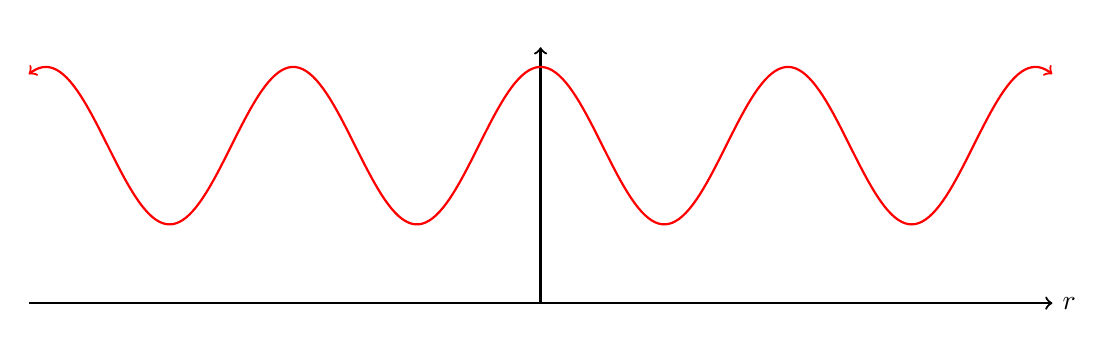
\begin{tikzpicture}[
	tl/.style = {% tick labels
		fill=white, inner sep=1pt, font=\scriptsize,},
	]
	
	% axes
	\draw[->,thick] (-6.5,-2) -- (6.5,-2) node[right] {$\vb{r}$};
	\draw[->,thick] (0,-2) -- (0, 1.25) node[above] {$$};
	% curve
	\draw[<->,thick,draw=red,
	domain=-6.5:6.5,samples=300,variable=\x] 
	plot (\x,{cos(deg{\x*2})});

\end{tikzpicture}

\begin{equation}
	H = \sum_i \left[\frac{\vb{P}_i^2}{2m} + U(\vb{r}_i)  \right]+ \sum_{ij} V_{e-e}^C (\vb{r}_i-\vb{R}j)
\end{equation}

\noindent This is, in general, a very hard problem to solve. In particular, it is the Coulomb-term which makes it really hard.\\
\linebreak

\noindent\uline{One-particle term:}
\begin{align}
	&H_1 = \sum_i H_1 (\vb{r}_i, \vb{P}_i)\\
	&H_1 (\vb{r}_i, \vb{P}_i) = \frac{\vb{P}_i^2}{2m} + U(\vb{r}_i)
\end{align}
\linebreak
\noindent \uline{Two-particle term:}
\begin{equation}
	H_2 = \sum_{ij} V_{e-e}^C (\vb{r}_i-\vb{R}j
\end{equation}

\noindent We will first work out the second-quantized form of the two terms in $H_1 (\vb{r}_i, \vb{P}_i)$. \\
\linebreak

\noindent We define $\varphi_\lambda ( \vb{r},s)$ as follows:
Solutions to the single-particle Schrödinger-equation

\begin{align}
	&H_1 \varphi_\lambda = \varepsilon_\lambda \varphi_\lambda\\
	&H_1 = -\frac{\hbar^2}{2m} \vb{\laplacian} + U(\vb{r}) ; \hspace{0.5cm} \vb{\laplacian} : \text{Laplace-operator} \label{h_1}
\end{align}

\noindent The task is now to find a second-quantized form of $H_1$ which will yield the \uline{same} matrix elements as \ref{h_1}.\\
\linebreak
\noindent Consider:
\begin{equation}
	\bra{\lambda_1} H_1 \ket{\lambda_2} ; \hspace{0.5cm} \braket{\lambda_1}{\lambda_2} = \delta_{\lambda_1, \lambda_2}
\end{equation}

\noindent \uline{Completeness relation:}

\begin{align}
	&\braket{\vb{r},s}{\lambda_1} = \varphi_{\lambda_{1}} \hspace{0.5cm} \text{(some wavefunction)} \nonumber\\
	&\text{Normalized states: } \braket{\lambda}{\lambda}=1 \nonumber \\
	&\sum_\lambda \varphi_\lambda^* (\vb{r},s) \varphi_\lambda (\vb{r'},s') = \delta(\vb{r}-\vb{r'}) \delta_{s,s'}\\
	&\sum_{\vb{r},s} \varphi_{\lambda'}^* (\vb{r},s) \varphi_\lambda (\vb{r},s) = \delta_{\lambda, \lambda'}\\
	& \braket{\lambda}{\lambda'}= \delta_{\lambda, \lambda'} \implies \sum_{\vb{r},s} \ket{\vb{r},s} \bra{\vb{r},s} = 1 ; \hspace{0.3cm} \sum_x \ket{x}\bra{x}=1
\end{align}

\noindent Now we use this version of the completeness relations to evaluate the matrix element $\bra{\lambda_1} H_1 \ket{\lambda_2}$

\begin{align}
	\bra{\lambda_1} H_1 \ket{\lambda_2} &= \sum_{\vb{r},s} \sum_{\vb{r'},s'} \braket{\lambda_1}{\vb{r},s} \bra{\vb{r},s} H_1 \ket*{\vb{r'},s'} \braket*{\vb{r'}}{\lambda_2}\\
	&=  \sum_{\vb{r},s} \sum_{\vb{r'},s'} \varphi_{\lambda_1}^* (\vb{r},s)  \bra{\vb{r},s} H_1 \ket*{\vb{r'},s'} \varphi_{\lambda_2} (\vb{r'},s') \nonumber
\end{align}

\begin{align}
	&H_1 = \frac{\vb{p}^2}{2m}+ U(\vb{r}) \hspace{1cm} \text{Classical}\\
	&\vb{p}= \frac{\hbar}{i} \vb{\gradient}  ;  \hspace{1cm} \vb{\gradient}: \text{Gradient operator}\\
	&H_1 =  - \frac{\hbar^2 \vb{\laplacian}}{2m} + U(\hat{r}) \hspace{1cm} \text{Quantum mechanical}\\
	& U(\hat{r}) \ket{r} = U(\vb{r})\ket{r}
\end{align}

\noindent $\vb{r}:$ Position : eigenvalue of the position operator

\begin{align}
	\hat{r} \ket{\vb{r},s}= \vb{r} \ket{\vb{r}, s}\\
	U(\hat{r}) \ket{\vb{r},s}= U(\vb{r}) \ket{\vb{r},s}
\end{align}


\begin{align}
	\bra{\vb{r},s} H_1 \ket*{\vb{r'},s'} &= \left[-\frac{\hbar^2}{2m} \vb{\laplacian}+ U(\vb{r}) \right] \delta_{\vb{r}, \vb{r'}} \delta_{s,s'}\\
	\bra{\lambda_1} H_1 \ket{\lambda_2} &= \sum_{\vb{r},s} \varphi_{\lambda_1}^* (\vb{r},s) \left[-\frac{\hbar^2}{2m} \vb{\laplacian}+ U(\vb{r}) \right] \varphi_{\lambda_2} (\vb{r},s)\\
	&\equiv \varepsilon_{\lambda_1, \lambda_2} \nonumber
\end{align}

\noindent $\varphi_\lambda (\vb{r},s): $ Some complete set of functions, by assumption.\\
\linebreak
\noindent Let us now give an alternative form of $H_1$, which will yield the \uline{same} matrix elements.
\linebreak
\noindent \uline{Anzats:}

\begin{equation}
	H_1 = \sum_{\lambda_1, \lambda_2} h_{\lambda_1, \lambda_2} \cd_{\lambda_1} c_{\lambda_2}
\end{equation}
where $ h_{\lambda_1, \lambda_2}$ is some complex number.
Then:
\begin{align}
	\bra{\lambda_1} H_1 \ket{\lambda_2} &= \bra{0}c_{\lambda_1} \left(\sum_{\lambda'_1, \lambda'_2} h_{\lambda'_1, \lambda'_2} \cd_{\lambda'_1} c_{\lambda'_2} \right) \cd_{\lambda_2} \ket{0} \\
	&=\sum_{\lambda'_1, \lambda'_2} h_{\lambda'_1, \lambda'_2}  \bra{0}c_{\lambda_1}  \cd_{\lambda'_1} c_{\lambda'_2} \cd_{\lambda_2} \ket{0} \nonumber \\
	&= \sum_{\lambda'_1, \lambda'_2} h_{\lambda'_1, \lambda'_2}  \bra{0} (\delta_{\lambda_1, \lambda'_1}-\cd_{\lambda'_1}c_{\lambda_1} ) (\delta_{\lambda_2, \lambda'_2} -\cd_{\lambda_2} c_{\lambda'_2}) \ket{0} \nonumber\\
	&= \sum_{\lambda'_1, \lambda'_2} h_{\lambda'_1, \lambda'_2}  \delta_{\lambda_1, \lambda'_1} \delta_{\lambda_2, \lambda'_2} \braket{0}{0}\nonumber \hspace{1cm} (c_\lambda \ket{0} =0)  \\
	&= h_{\lambda_1, \lambda_2} \nonumber
\end{align}
Choose $ h_{\lambda_1, \lambda_2} = \varepsilon_{\lambda_1, \lambda_2}$ $\implies$ Same matrix-elements for
\begin{equation}
	H_1 = -\frac{\hbar^2}{2m} \vb{\laplacian}+ U(\hat{r}) 
\end{equation}
and
\begin{tcolorbox}
	\begin{equation}
		H_1 = \sum_{\lambda_1, \lambda_2} \varepsilon_{\lambda_1, \lambda_2} \cd_{\lambda_1} c_{\lambda_2} \label{sec_quant_h}
	\end{equation}
\end{tcolorbox}
Thus, \ref{sec_quant_h} is a useful 2nd quantized form of $H_1$.\\
\linebreak
\noindent This expression may be simplified. Consider now a judicial choice of the complete set $\{\varphi_\lambda(x) \}$:\\
\noindent Let ${\varphi_\lambda}$ be defined by

\begin{equation}
	\left(-\frac{\hbar^2}{2m} \vb{\laplacian}+ U(\vb{r})  \right) \varphi_\lambda(x) = \varepsilon_\lambda \varphi_\lambda(x)
\end{equation}
i.e. ${\varphi_\lambda}$ are eigenfunctions of $H_1$\\
\linebreak
\noindent Then:
\begin{align}
	\varepsilon_{\lambda_1, \lambda_2} &= \sum_x \varphi_{\lambda_1}^*(x)  \left(-\frac{\hbar^2}{2m} \vb{\laplacian}+ U(\vb{r})  \right) \varphi_{\lambda_2} (x)\\
	&=  \sum_x \varphi_{\lambda_1}^*(x) \varepsilon_{\lambda_2} \varphi_{\lambda_2}(x) \nonumber \\
	&= \varepsilon_{\lambda_2} \sum_x \varphi_{\lambda_1}^*(x) \varphi_{\lambda_2}(x)\nonumber \\
	&= \varepsilon_{\lambda_2} \delta_{\lambda_1, \lambda_2} \nonumber
\end{align}
giving that, 
\begin{equation}
	H_1 = \sum_{\lambda_1} \varepsilon_{\lambda_1} \cd_{\lambda_1} c_{\lambda_1}
\end{equation}

\noindent This form of $H_1$ has an intuitively appealing form: $  \cd_{\lambda_1} c_{\lambda_1}$ is a number operator. It counts the number of particles in state $\ket{\lambda_1}$.\\
\noindent $\varepsilon_\lambda$ is the single-particle energy in this state. Thus, $H_1$ is an operator that counts the energy in the system coming from all the possible states of the system.\\
\linebreak
\noindent General one-particle operators:
\begin{equation}
	T(x, \vb{p}) = T(x, \frac{\hbar}{i} \vb{\gradient}) 
\end{equation}
Could in principle depend on spin-coordinate $s$ !
\begin{equation}
	\bra{\lambda_1} T \ket{\lambda_2} = \sum_x \varphi_{\lambda_1}^*(x) T(x, \frac{\hbar}{i} \vb{\gradient}) \varphi_{\lambda_2}(x)
\end{equation}

\begin{tcolorbox}
	\begin{align}
		T &= \sum_{\lambda_1,\lambda_2} \bra{\lambda_1} T(x, \vb{p}) \ket{\lambda_2} \cd_{\lambda_1} c_{\lambda_2}\\
		&=\sum_{\lambda_1,\lambda_2} t_{\lambda_1,\lambda_2} \cd_{\lambda_1} c_{\lambda_2} \nonumber
	\end{align}
\end{tcolorbox}
\noindent This expression for $H_1$ and $T$ in second quantized form applies for any choice of sets of quantum numbers $\lambda$.\\
\linebreak
\noindent We next proceed by setting up a general form of second quantized form of 2-particle operators.


\begin{equation}
	H= \sum_i H_1(\vb{p}_i, \vb{r}_i) + \sum_{i,j} H_2 (\vb{r}_i, \vb{r}_j )
\end{equation}

\begin{tcolorbox}
	\noindent Second-quantized form (general):
	
	\begin{align}
		H & = \sum_{\lambda_{1}, \lambda_{2}} \bra{\lambda_{1}} H_1 \ket{\lambda_{2}} \cd_{\lambda_1} c_{\lambda_2} \nonumber \\
		&+ \sum_{\lambda_{1}} \cdots \sum_{\lambda_{4}} \bra{\lambda_{1}, \lambda_{2}} H_2 \ket{\lambda_{3}, \lambda_{4}} \cd_{\lambda_1} \cd_{\lambda_2} c_{\lambda_{3}} c_{\lambda_{4}}
	\end{align}
\end{tcolorbox}
%\linebreak

\subsection{Plane-wave basis}

\noindent i) \uline{Plane-wave basis:}  ${\varphi_{\lambda} (\vb{r},s) = \frac{1}{\sqrt{V}} \e^{i \vb{k}\cdot \vb{r}} \chi_\sigma (s)  }$ \\
\linebreak

\noindent \uline{Completeness:}

\begin{equation}
	\sum_{\vb{k}} \sum_{\sigma} \varphi_{\vb{k}, \sigma}^* (\vb{r}', s') \varphi_{\vb{k}, \sigma} (\vb{r}, s) = \delta_{\vb{r}, \vb{r}'} \delta_{s,s'}
\end{equation}
\linebreak
\noindent \uline{Orthogonality:}

\begin{equation}
	\sum_{\vb{r}} \sum_{s} \varphi_{\vb{k}', \sigma'}^* (\vb{r}, s) \varphi_{\vb{k}, \sigma} (\vb{r}, s) = \delta_{\vb{k}, \vb{k}'} \delta_{\sigma,\sigma'}
\end{equation}
\linebreak
\noindent Field-operators are given by

\begin{equation}
	\psi^\dagger (\vb{r},s,t) = \sum_{\vb{k}, \sigma} \cd_{\vb{k}, \sigma} (t) \left( \frac{1}{\sqrt{V}} \e^{i \vb{k} \cdot \vb{r}} \chi_\sigma (s) \right)
\end{equation}

\begin{align}
	&\{c_{k,\sigma}(t), \cd_{ k', \sigma'} \}= \delta_{k,k'}\delta_{\sigma,\sigma'}\\
	&\{c_{k,\sigma}(t), c_{ k', \sigma'} \}= 0\\
	&\{\cd_{k,\sigma}(t), \cd_{ k', \sigma'} \}= 0
\end{align}

\noindent Orthonormality, spatial part

\begin{equation}
	\frac{1}{V} \sum_{\vb{r}} \e^{i \vb{r}\cdot (\vb{k}-\vb{k}')} = \delta_{\vb{k}, \vb{k}'}
\end{equation}

\noindent Orthonormality, spin part

\begin{equation}
	\sum_s \chi_{\sigma_1}^* (s) \chi_{\sigma_2} (s) = \delta_{\sigma_1,\sigma_2}
\end{equation}

\noindent Completeness, spatial part

\begin{equation}
\frac{1}{V} \sum_{\vb{k}} \e^{i \vb{k}\cdot (\vb{r}-\vb{r}')} = \delta_{\vb{r}, \vb{r}'}
\end{equation}

\noindent Completeness, spin part

\begin{equation}
\sum_{\sigma} \chi_{\sigma}^* (s') \chi_{\sigma} (s) = \delta_{s',s}
\end{equation}

\noindent The plane-waves are eigenfunctions of $H_{10} \equiv -\frac{\hbar^2}{2m} \vb{\laplacian}$ $\implies$

\begin{align}
	& H_{10} = \sum_{\vb{k}_1, \sigma_1} \sum_{\vb{k}_2, \sigma_2} \bra*{\vb{k}_1, \sigma_1} H_{10} \ket*{\vb{k}_2, \sigma_2} \cd_{ \vb{k}_1, \sigma_1} c_{\vb{k}_2, \sigma_2}\\
	&  \bra*{\vb{k}_1, \sigma_1} H_{10} \ket*{\vb{k}_2, \sigma_2}  = \frac{1}{V} \sum_{\vb{r}} \e^{i (\vb{k}_1-\vb{k}_2)\cdot \vb{r}}  \sum_s \chi_{\sigma_1}^*(s) \chi_{\sigma_2}(s) \frac{\hbar^2 k_2^2}{2m}\\
	& H_{10}= \sum_{\vb{k_1}, \sigma_1} \frac{\hbar^2 k_1^2}{2m} \cd_{ \vb{k}_1, \sigma_1} c_{ \vb{k}_1, \sigma_1} \nonumber\\ 
	& H_{10}= \sum_{\vb{k}, \sigma} \varepsilon_k \cd_{k \sigma} c_{ k, \sigma} \hspace{0.1cm} ; \hspace{0.5cm} \varepsilon_k = \frac{\hbar^2 k^2}{2m} \nonumber
\end{align}

\noindent The next contribution to $H_1$ is the crystal potential $U(\vb{r}_i)= H_{11}(r_i)$\\
$ \sum_i U(\vb{r}_i) \rightarrow \sum_{\lambda_{1}, \lambda_{2}} \bra{\lambda_{1}}H_{11} \ket{\lambda_{2}} \cd_{ \vb{k}_1, \lambda_1} c_{\lambda_{2}}$

\begin{align}
	\bra{\lambda_{1}} H_{11} \ket{\lambda_{2}} &= \sum_{\vb{r}} \sum_s \frac{1}{\sqrt{V}} \e^{-i \vb{k}_1\cdot \vb{r}} \chi_{\sigma_1}^*(s) U(\vb{r}) \frac{1}{\sqrt{V}} \e^{i \vb{k}_2 \cdot \vb{r}} \chi_{\sigma_2}(s)\\
	&= \frac{1}{V} \sum_{\vb{r}} \e^{i (\vb{k}_2-\vb{k}_1) \cdot \vb{r}} U(\vb{r}) \sum_s \chi_{\sigma_1}^* (s) \chi_{\sigma_2}(s) \nonumber 
\end{align}

\noindent Introduce Fourier-transform of the crystal-potential

\begin{align}
	\tilde{U}(\vb{q}) &\equiv \frac{1}{V} \sum_{\vb{r}} \e^{-i \vb{q}\cdot \vb{r}} U(\vb{r})\\
	U(\vb{r}) &= \sum_{\vb{q}} \tilde{U}(\vb{q}) \e^{i \vb{q} \vb{r}}
\end{align}

\begin{equation}
	\bra{\lambda_{1}} H_{11} \ket{\lambda_{2}}= \delta_{\sigma_1,\sigma_2} \tilde{U}(\vb{k}_1-\vb{k}_2)
\end{equation}


\begin{align}
	\sum_{\lambda_{1}} \sum_{\lambda_{2}} 	\bra{\lambda_{1}} H_{11} \ket{\lambda_{2}} \cd_{\lambda_1} c_{\lambda_{2}} &= \sum_{\vb{k}_1} \sum_{\vb{k}_2} \sum_{\sigma} \tilde{U}(\vb{k}_1-\vb{k}_2) \cd_{ \vb{k}_1, \sigma} c_{\vb{k}_2, \sigma} \nonumber \\
	&= \sum_{\vb{k}, \vb{q}, \sigma} \tilde{U} (\vb{q}) \cd_{ \vb{k}+\vb{q}, \sigma} c_{\vb{k}, \sigma} \nonumber
\end{align}

\noindent Where we have defined $\vb{q} \equiv \vb{k}_1- \vb{k}_2$ ; $\vb{k}_2 \equiv \vb{k}$.\\
\linebreak
\noindent Scattering of plane-waves $\ket*{\vb{k}, \sigma} \rightarrow \ket*{\vb{k}+\vb{q}, \sigma}$ by crystal lattice. Momentum $\vb{q}$ is transferred to fermions (electrons) from the lattice. Spin is conserved in the scattering. 

\begin{align}
	H_1 &= \sum_i \left[ \frac{p_i^2}{2m}+U(\vb{r}_i) \right] \implies \\
	H_1 &= \sum_{\vb{k}, \sigma} \varepsilon_k \cd_{k, \sigma} c_{k, \sigma} +\sum_{\vb{k},\vb{q}, \sigma} \tilde{U}(\vb{q})  \cd_{ k+q, \sigma} c_{k,\sigma} \hspace{0.5cm} ; \hspace{0.2cm} \varepsilon_k= \frac{\hbar^2 k^2}{2m}
\end{align}


\begin{figure}[!h]
	\centering
		\begin{tikzpicture}%[scale=3]
			%\itshape
			\begin{feynman}[large]
				\vertex[small,dot](a){};
				\vertex [right= of a](b);
				\vertex [above left=of a](i1);
				\vertex [below left=of a](i2);
				
				\node[anchor = east] at ($(a)+(+0.1,0)$) ;
				\diagram{
				(b) --[scalar, edge label' = $\tilde{U}(\vb{q})$] (a) ,
				(i2)--[fermion, edge label' ={\(\vb{k}, \sigma\)}] (a) -- [fermion, edge label'={\(\vb{k}+\vb{q}, \sigma\)}] (i1), 	
				};
			\end{feynman}
	
		\end{tikzpicture}
	\caption*{Illustration of the scattering event}
\end{figure}

\noindent Next, we second-quantize the Coulomb interaction in the plane-wave basis.\\
\linebreak
\noindent Electron-electron interaction:


\begin{equation}
	H_2 = \sum_{\lambda_{1}}\cdots \sum_{\lambda_{4}} \bra{\lambda_{1}, \lambda_{2}}V_{e-e}^C \ket{\lambda_{3},\lambda_{4}} \cd_{\lambda_1} \cd_{\lambda_2} c_{\lambda_{3}} c_{\lambda_4}
\end{equation}

\begin{align}
	&\bra{\lambda_{1}, \lambda_{2}}V_{e-e}^C (\vb{r}_i-\vb{r}_j) \ket{\lambda_{3},\lambda_{4}} \\
	&= \sum_{s_1} \cdots \sum_{s_4} \chi_{\sigma_1}^* (s_1) \chi_{\sigma_2}^*(s_2) \chi_{\sigma_3}(s_3) \chi_{\sigma_4}(s_4) \nonumber\\
	& \cdot \frac{1}{V^2} \sum_{\vb{r}_1 \cdots \vb{r}_4} \e^{-i \vb{k}_1 \vb{r}_1- i \vb{k}_2 \cdot \vb{r}_2 + i \vb{k}_3\cdot \vb{r}_3+ i \vb{k}_4 \cdot \vb{r}_4  }  \nonumber \\ 
	& \cdot V_{e-e}^C (\vb{r}_3- \vb{r}_4) \delta_{s_2, s_3} \delta_{s_1, s_4} \delta_{\vb{r}_2, \vb{r}_3} \delta_{\vb{r}_1, \vb{r}_4}\nonumber 
\end{align}

\noindent Spin-part: Four sums over s's reduce to two:

\begin{equation*}
	\sum_{s_1} \sum_{s_2}  \chi_{\sigma_1}^* (s_1) \chi_{\sigma_2}^*(s_1) \chi_{\sigma_3}(s_2) \chi_{\sigma_4}(s_2) = \delta_{\sigma_1,\sigma_2} \delta_{\sigma_3, \sigma_4}
\end{equation*}

\noindent Spatial part: Again, four sums over $\vb{r}$ reduce to 2: 

\begin{equation*}
	\sum_{\vb{r}_1} \sum_{\vb{r}_2} V_{e-e}^C (\vb{r}_2-\vb{r}_1) \frac{1}{V^2} \e^{i (\vb{k}_4-\vb{k}_1)\cdot \vb{r}_1} \e^{i (\vb{k}_3-\vb{k}_2)\cdot \vb{r}_2} 
\end{equation*}
\noindent Rewrite plane-wave factors in such a way that we can factor out a Fourier-transform of $V_{e-e}^C (\vb{r}_2-\vb{r}_1)$. We therefore need a plane-wave factor of the type $\e^{i \vb{q}\cdot (\vb{r}_2- \vb{r}_1)}$. Since the spatial argument of $V_{e-e}^C$ is $\vb{r}_2 -\vb{r}_1$ here.

\begin{equation*}
	\e^{i (\vb{k}_4-\vb{k}_1)\cdot \vb{r}_1} \e^{i (\vb{k}_3-\vb{k}_2)\cdot \vb{r}_2}  = \e^{i(\vb{k}_4-\vb{k}_1+ \vb{k}_3-\vb{k}_2)\cdot \vb{r}_1} \e^{i(\vb{k}_3- \vb{k}_2) \cdot (\vb{r}_2- \vb{r}_1)}
\end{equation*}

\noindent Define $\vb{r}_2 -\vb{r}_1 \equiv \vb{r}$ and sum over $(\vb{r}, \vb{r}_1)$ instead of $(\vb{r}_1, \vb{r}_2)$

\begin{align*}
	\sum_{\vb{r}} V_{e-e}^C \e^{i(\vb{k}_3-\vb{k}_2)\cdot \vb{r}} \frac{1}{V^2} \sum_{\vb{r}_1} \e^{i(\vb{k}_3+\vb{k}_4-\vb{k}_1-\vb{k}_2)\cdot \vb{r}_1} &=\sum_{\vb{r}} V_{e-e}^C \e^{i(\vb{k}_3-\vb{k}_2)\cdot \vb{r}}   \frac{1}{V} \delta_{\vb{k}_3+\vb{k}_4, \vb{k}_1+\vb{k}_2}\\
	&= \tilde{V}_{e-e}^C (\vb{k}_2-\vb{k}_3) \delta_{\vb{k}_3+\vb{k}_4, \vb{k}_1+\vb{k}_2}
\end{align*}

\noindent Fourier-transform of Coulomb-potential: 

\begin{align*}
	\tilde{V}_{e-e}^C (\vb{q})  \equiv \frac{1}{V} \sum_{\vb{r}} \e^{-i \vb{q} \cdot \vb{r} } V_{e-e}^C (\vb{r})
\end{align*}


\noindent Thus, we have so far

\begin{align*}
	H_2 = \sum_{\vb{k}_1...\vb{k}_4 } \sum_{\sigma_1, \sigma_2} \tilde{V}_{e-e}^C (\vb{k}_2- \vb{k}_3) \delta_{\vb{k}_3+\vb{k}_4, \vb{k}_1+\vb{k}_2} \cd_{ \vb{k}_1, \sigma_1} \cd_{ \vb{k}_2, \sigma_2}  c_{ \vb{k}_3, \sigma_2} c_{ \vb{k}_4, \sigma_1},
\end{align*}

defining $\vb{q} \equiv \vb{k}_2- \vb{k}_3 \implies \vb{k}_3 =  \vb{k}_2-\vb{q}, \hspace{0.4cm} \vb{k}_4 = \vb{k}_1 + \vb{k}_2-\vb{k}_3 = \vb{k}_1- \vb{q}$.
Thus, sum over $\vb{k}_1, \vb{k}_2, \vb{q}$:

\begin{align*}
H_2 = \sum_{\vb{k}_1,\vb{k}_2,\vb{q} } \sum_{\sigma_1, \sigma_2} \tilde{V}_{e-e}^C (\vb{q}) \cd_{ \vb{k}_1, \sigma_1} \cd_{ \vb{k}_2, \sigma_2}  c_{ \vb{k}_3-\vb{q}, \sigma_2} c_{ \vb{k}_1+\vb{q}, \sigma_1}
\end{align*}

\noindent This is a scattering process between two electrons. 
\noindent Diagrammatically, we may view the scattering event as: 

 
\begin{center}
	\begin{tikzpicture}
	\begin{feynman}[large]
	\vertex (a); 
	\vertex[left= 3 cm of a] (b);
	\vertex[above left= 3cm of b] (c); 
	\vertex[below left= 3 cm of b] (d); 
	\vertex[above right= 3cm of a] (f1); 
	\vertex[below right= 3cm of a] (f2); 
	\diagram*{(b) --[charged boson, edge label = \(\vb{q}\)] (a), (b) --[fermion, edge label' = \( \vb{k}_1  \comma \sigma_1\)] (c), 
		(b) --[anti fermion, edge label = \(\vb{k}_1+\vb{q} \comma \sigma_1\)] (d), (a) --[fermion, edge label = \(\vb{k}_2 \comma \sigma_2\)] (f1), (a) --[anti fermion, edge label' = \(\vb{k}_2-\vb{q} \comma \sigma_2\)] (f2),
	}; 
	\node[anchor = west] at (-5,0) {};
	\node[anchor = west] at (0.2,0) {};
	\node[] at (-1.5,-0.6) {$\tilde{V}_{e-e}^C (\vb{q})$};
	\end{feynman}
	\end{tikzpicture}
\end{center}

\noindent Note that the spin of each electron is conserved in the scattering, since Coulomb-interaction is a purely electrostatic, spin-independent potential. This in total, we have

\begin{align*}
	H &= \sum_{\vb{k}, \sigma} \varepsilon_{\vb{k}} \cd_{ \vb{k}, \sigma} c_{\vb{k}, \sigma} +  \sum_{\vb{k}, \vb{q} \sigma} \tilde{U}(\vb{q}) \cd_{ \vb{k}+\vb{q}, \sigma}c_{\vb{k}, \sigma}\\
	& +  \sum_{\vb{k}_1,\vb{k}_2,\vb{q} } \sum_{\sigma_1, \sigma_2} \tilde{V}_{e-e}^C (\vb{q}) \cd_{ \vb{k}_1, \sigma_1} \cd_{ \vb{k}_2, \sigma_2}  c_{ \vb{k}_3-\vb{q}, \sigma_2} c_{ \vb{k}_1+\vb{q}, \sigma_1}
\end{align*}

\noindent For a static crystal, $\tilde{U}(\vb{q})$ is some given fixed external potential that electrons move in. In that case, it is the Coulomb term which makes the problem really hard, since it represents a genuine many-particle problem. On the other hand, if the lattice it self has dynamics, then this introduces additional scattering of electrons, now off quantized lattice vibrations (phonons). In that case, the second term involving $\tilde{U}(\vb{q})$ will include phonons, and this turns the $\tilde{U}(\vb{q})$- term also into a genuine many-body problem. We will later in the course return to the important problem of studying coupling between electrons and phonons.\newline

\subsection{Atomic orbital basis}

\noindent ii) \uline{Atomic orbital basis (lattice fermions)}

\noindent We now consider a system where fermions most of the time stay localized on sites on a lattice. Occasionally, they may tunnel from one lattice site to another. This tunneling arises because the long-distance (away from lattice sites) tails of the atomic orbitals (Wannier-functions) may overlap.

\begin{center}
	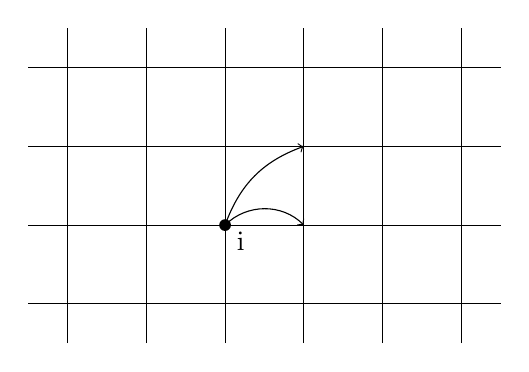
\begin{tikzpicture}
		\draw[step=1.0,black,thin] (0.5,0.5) grid (6.5,4.5);	
		\draw[->] (3,2)  to [out=70,in=200, looseness=1] (4,3);
		\draw[->] (3,2)  to [out=45,in=135, looseness=1] (4,2);
		\node at (3,2) [circle,fill,inner sep=1.5pt]{};
		\node at (3.2,1.8) {i};
	\end{tikzpicture}
\end{center}
\noindent Two tunneling processes ("hopping") on a 2D rectangular lattice, from lattice site \uline{i} to its \uline{nearest} and \uline{next-nearest} neighbors. The long distance tails of the Wannier-functions fall off exponentially (recall the wave-functions of the Hydrogen-atom). Therefore, hopping is most likely to occur from a lattice site i to its nearest neighbor. The next most probable hopping event is a direct hopping from i to its next-nearest neighbor, or two hopping via an intermediate nearest neighbor. Which process is most likely is a matter of some detail: The two factors that mostly determine this is the distance between atoms on the lattice, and the type of atoms which are situated on the lattice points. If $\Delta \vb{r}$ is the separation between the electron and the ionic position, then the Wannier-functions fall off approximatly as $\e^{-\Delta \vb{r}/\lambda}$
\begin{align*}
	\lambda = c \frac{a_0}{Z}
\end{align*}

\noindent $c$: Constant of order unity \newline
\noindent $a_0$: Bohr-radius\newline
\noindent $Z$: Number of protons in the nucleus\newline

\noindent For heavy atoms, Wannier orbitals are more tightly localized around atoms than in lighter elements. \newline
Crystal potential (rigid crystal) \newline

\noindent $U= \sum_i U(\vb{r}_i) $ \\
\noindent $U(\vb{r}_i)= \sum_j U(\vb{r}_i, \vb{R}j)$\\
\noindent $\vb{r}_i$: Electronic coordinate ; $\vb{R}j$: Ionic coordinate.\\

\noindent $U_a(\vb{r}_i, \vb{R}j)$: Potential energy that electron at $\vb{r}_i$ feels from ion located at $\vb{R}j$. The dominant contribution to this is when $i=j$, i.e. when the electron and ion is on the same site $i$. We single out this contribution as follows
\begin{align*}
	U = \sum_i U_a(\vb{r}_i, \vb{r}_i) + \sum_i \sum_{j\neq i}  U_a(\vb{r}_i, \vb{R}j).
\end{align*}
\noindent The point of this splitting is that the basis functions $\{\varphi_\lambda \}$ that we will choose, will be the eigenfunctions of the total Hamilton-operator for \uline{isolated} atoms. This is a very natural choice for a system where electrons spend most of the time on isolated atoms and only relatively rarely hop from one site to the other.\newline

\noindent Schrödinger-equation for isolated atoms:

\begin{align*}
	\left[\frac{\vb{p}_i^2}{2m}+ U_a( \vb{r}_i, \vb{R}_i)\right] \varphi_{\alpha, \sigma}( \vb{r}_i, s_i)= \varepsilon_{\alpha,\sigma, i} \varphi_{\alpha, \sigma}( \vb{r}_i, s_i)
\end{align*}

\noindent $\alpha$: Index for atomic orbital \\
\noindent $\sigma$: Spin quantum number\\
\noindent $\vb{r}_i$: Spatial coordinate of electron on lattice site $i$\\
\noindent $\s_i$: Spin-coordinate of electron on lattice site $i$r\\
\noindent $\varepsilon_{\alpha,\sigma, i}$: Energy of electron in orbital $\alpha$ on lattice site$i$. In principle this energy could vary from lattice site to lattice site, but for most systems we will let $\varepsilon_{\alpha, \sigma, i} = \varepsilon_{\alpha, \sigma}$ i.e. independent of the position on the lattice. In principle, $\varepsilon_{\alpha, \sigma}$ could depend on spin. 
If we now bring in the rest of the crystal potential (from the surrounding atoms) in the one-particle Hamiltonian, the basis set $\{\varphi_\lambda \}$ that we have chosen, are no longer eigenfunctions of the Hamiltonian. This leads to scattering from one state $\ket{\lambda}$ to another state $\ket{\lambda'}$, and this in term gives rise to tunneling, or hopping, of electrons on the lattice. Thus, the hopping of electrons around on the lattice, which represents kinetic energy, originates with the crystal potential from surrounding atoms working on an electron. The details are as follows:

\begin{align*}
	&\varphi_{\alpha, \sigma,j}(\vb{r}_i,s_i) = \Phi_{\alpha, j}^W (\vb{r}_i) \cdot \chi_\sigma (s_i)\\
	&\lambda = (\alpha, \sigma, j)
\end{align*}
(\uline{Note}: $\alpha$ must be thought of as consisting of two numbers: (l,m) of a hydrogen-like atom.)\\

\noindent Field operator:
\begin{align*}
	\psi^\dagger_j(\vb{r}_i, s_i, t)= \sum_{\alpha, \sigma} \cd_{\alpha, \sigma, i} \Phi_{\alpha, j}^* (\vb{r}_i) \cdot \chi^*_\sigma (s_i)
\end{align*}
\begin{align*}
	\{ c_{\alpha, \sigma, i},\cd_{\alpha', \sigma', i'} \} = \delta_{\alpha, \alpha'} \delta_{\sigma,\sigma'} \delta_{i,i'}
\end{align*}
Other commutators are zero.\\

\noindent \uline{Orthogonality}:

\begin{align*}
	\sum_{\vb{r}} \sum_s  \varphi^*_{\alpha, \sigma,j}(\vb{r},s)\varphi_{\alpha', \sigma',j'}(\vb{r},s) \approx \delta_{\alpha, \alpha'} \delta_{\sigma,\sigma'} \delta_{j,j'}
\end{align*}

\noindent \uline{Completeness}:

\begin{align*}
\sum_{\alpha, \sigma, j} \varphi^*_{\alpha, \sigma,j}(\vb{r},s)\varphi_{\alpha, \sigma,j}(\vb{r}',s') \approx \delta_{\vb{r},\vb{r}'} \delta_{s,s'} 
\end{align*}

\begin{align*}
	H_1 = \sum_i \left( \frac{\vb{p}_i^2}{2m}+ U_a (\vb{r}_i, \vb{R}_i) \right) + \sum_i \sum_{j \neq i} U_a ( \vb{r}_i, \vb{R}_j)
\end{align*}

\noindent Since the basis-functions are assumed to be eigenfunctions of the first term, we have:

\begin{align*}
	&\sum_i  \frac{\vb{p}_i^2}{2m}+ U_a (\vb{r}_i, \vb{R}_i)\\
	\implies & \sum_{\alpha, \sigma, i} \varepsilon_{\alpha, \sigma, i} \cd_{\alpha, \sigma, i} c_{\alpha, \sigma, i}
\end{align*}

\noindent Consider now the term

\begin{align*}
	& \sum_i \sum_{j \neq i} U_a ( \vb{r}_i, \vb{R}_j)\\
	\implies & H_{12} = \sum_{{\lambda_{1}}, {\lambda_{2}}} \bra{\lambda_{1}}  \sum_{j \neq i} U_a ( \vb{r}_i, \vb{R}_j) \ket{\lambda_{2}} \cd_{ \lambda_1} c_{\lambda_{2}}\\
	&= \sum_{\alpha_1, \sigma_1, i_1} \sum_{\alpha_2, \sigma_2, i_2} \bra{\alpha_1, \sigma_1, i_1} \sum_{j \neq i_2} U_a \ket{\alpha_2, \sigma_2, i_2} \cd_{\alpha_1, \sigma_1, i_1} c_{\alpha_2, \sigma_2, i_2}
\end{align*}

The matrix element: 

\begin{align*}
	&\bra{\alpha_1, \sigma_1, i_1} \sum_{j \neq i_2} U_a \ket{\alpha_2, \sigma_2, i_2}\\
	&= \sum_s \sum_{\vb{r}} \varphi_{\alpha_1, \sigma_1, i_1} (\vb{r},s) \underbrace{\left[\sum_j U_a (\vb{r},\vb{R}_j) \right] }_{\mathclap{\text{Sum from surrounding atoms}}}  \varphi_{\alpha_2, \sigma_2, i_2}(\vb{r},s)
\end{align*}

Here, we have used
